\documentclass[a4paper,titlepage,12pt]{article}
\usepackage[utf8]{inputenc} %Make sure all UTF8 characters work in the document
\usepackage{graphicx}
\usepackage{titling}
\usepackage{tabularx}
\usepackage{longtable}
\usepackage[yyyymmdd]{datetime}
\usepackage[figurename=Figur]{caption}
\usepackage{booktabs}
\usepackage[parfill]{parskip}
\usepackage{xcolor}

\lstdefinestyle{DOS}
{
	backgroundcolor=\color{black},
	basicstyle=\scriptsize\color{white}\ttfamily
}

%Set page size
\usepackage{geometry}
\geometry{margin=3cm}

\renewcommand{\dateseparator}{-}
\renewcommand{\contentsname}{Innehållsförteckning}
\renewcommand{\tablename}{Tabell}


\usepackage{listings}
\usepackage{color}

\usepackage[colorinlistoftodos,prependcaption,textsize=tiny]{todonotes}

\definecolor{dkgreen}{rgb}{0,0.6,0}
\definecolor{gray}{rgb}{0.5,0.5,0.5}
\definecolor{mauve}{rgb}{0.58,0,0.82}

\lstset{frame=tb,
  language=Python,
  aboveskip=3mm,
  belowskip=3mm,
  showstringspaces=false,
  columns=flexible,
  basicstyle={\small\ttfamily},
  numbers=none,
  numberstyle=\tiny\color{gray},
  keywordstyle=\color{blue},
  commentstyle=\color{dkgreen},
  stringstyle=\color{mauve},
  breaklines=true,
  breakatwhitespace=true,
  tabsize=3
}

%%%%%%%%%%%%%%%%%%%%%%%%%%%%%%%
% Header and footer
%%%%%%%%%%%%%%%%%%%%%%%%%%%%%%%
\usepackage{fancyhdr}
\pagestyle{fancy}

\lhead{
\includegraphics[width=0.15\linewidth]{../images/logo_full.png}}
\chead{Teknisk manual för sexbent robot}
\rhead{\today}
\setlength\headheight{26pt} 

\lfoot{TSEA29 -- KMM \\ LIPS Teknisk Manual}
\rfoot{Grupp 9 \\ LiTHe Hex}

\newcommand{\itc}{I\textsuperscript{2}C}

\pretitle{%
	\begin{center}
		\LARGE
		
\includegraphics[width=6cm]{../images/logo_full.png}\\[\bigskipamount]
}

\posttitle{\end{center}}

\begin{document}
\listoftodos
	\title{\LARGE
		\textbf{Teknisk manual för sexbent robot} \\
		\vspace*{0.5\baselineskip}
		\large
		Redaktör ??? \\
		Grupp 9 \\
		\small
		\vspace*{0.5\baselineskip}
		Version 0.1}

	\date{\today}

	\maketitle
	
	\newpage

	\tableofcontents
	\newpage


	%%%%%%%%%%%%%%%%%%%%%%%%%%%%%%%%%%%%%%%%%%%%%%%%%%%%%%%%%%%%%%%%%%%%%%%%%%%%%%%%%
	%						Historik
	%%%%%%%%%%%%%%%%%%%%%%%%%%%%%%%%%%%%%%%%%%%%%%%%%%%%%%%%%%%%%%%%%%%%%%%%%%%%%%%%%

	\section*{Dokumenthistorik}
	\renewcommand*{\arraystretch}{1.4}
    \begin{longtable}[c]{ l l >{\raggedright}p{5cm} >{\raggedright}p{3cm} l }
		\textbf{Version} & \textbf{Datum} & \textbf{Utförda förändringar} 
		& \textbf{Utförda av} & \textbf{Granskad} \\ \midrule
		
		0.1 & 2016--10--20 & Första utkastet & Projektgruppen &
        Projektgruppen \\
            
	\end{longtable}

	%%%%%%%%%%%%%%%%%%%%%%%%%%%%%%%%%%%%%%%%%%%%%%%%%%%%%%%%%%%%%%%%%%%%%%%%%%%%%%%%%
	%						Inledning
	%%%%%%%%%%%%%%%%%%%%%%%%%%%%%%%%%%%%%%%%%%%%%%%%%%%%%%%%%%%%%%%%%%%%%%%%%%%%%%%%%

	\newpage

	\raggedright

	\section{Inledning}
	Detta dokument går i detalj in på konstruktionen och mjukvaran för en 
	sexbent robot, med autonom och manuell styrning. Först presenteras en 
	översiktlig beskrivning av robotens styrande processorer ("enheter", vilka kopplas till ett färdigt 
	PhantomX AX Metal Hexapod Mark III chassi från TrossenRobotics). Dessa (central-, 
	motorik- och sensorenhet), kommunikation mellan dessa, samt användargränssnitt specificeras 
	sedan i större noggrannhet under egna avdelningar.

	%%%%%%%%%%%%%%%%%%%%%%%%%%%%%%%%%%%%%%%%%%%%%%%%%%%%%%%%%%%%%%%%%%%%%%%%%%%%%%%%%
	%						Översikt
	%%%%%%%%%%%%%%%%%%%%%%%%%%%%%%%%%%%%%%%%%%%%%%%%%%%%%%%%%%%%%%%%%%%%%%%%%%%%%%%%%
	
    \newpage
	\section{Centralenheten}
	

	%%%%%%%%%%%%%%%%%%%%%%%%%%%%%%%%%%%% %%%%%%%%%%%%%%%%%%%%%%%%%%%%%%%%%%%%%%%%%%%%%
	%						Motorikenheten
	%%%%%%%%%%%%%%%%%%%%%%%%%%%%%%%%%%%%%%%%%%%%%%%%%%%%%%%%%%%%%%%%%%%%%%%%%%%%%%%%%
    \newpage
	\section{Motorikenheten}
	
	

	%%%%%%%%%%%%%%%%%%%%%%%%%%%%%%%%%%%%%%%%%%%%%%%%%%%%%%%%%%%%%%%%%%%%%%%%%%%%%%%%%
	%						Sensorenheten
	%%%%%%%%%%%%%%%%%%%%%%%%%%%%%%%%%%%%%%%%%%%%%%%%%%%%%%%%%%%%%%%%%%%%%%%%%%%%%%%%%
	\section{Sensorenheten}

	
	%%%%%%%%%%%%%%%%%%%%%%%%%%%%%%%%%%%%%%%%%%%%%%%%%%%%%%%%%%%%%%%%%%%%%%%%%%%%%%%%%
	%						Grafiskt användargränssnitt
	%%%%%%%%%%%%%%%%%%%%%%%%%%%%%%%%%%%%%%%%%%%%%%%%%%%%%%%%%%%%%%%%%%%%%%%%%%%%%%%%%

    \newpage
	\section{Grafiskt användargränssnitt}
	Här beskrivs hur man använder det grafiska användargränssnittet för roboten.
	
	\subsection{Starta webbservern}
	Man startar servern genom att gå till mappen "/var/www/gui/" och skriva "mix phoenix.server". Se exempel nedan:
	
	\begin{lstlisting}[style=DOS]
	Microsoft Windows [Version 6.1.7601]
	Copyright (c) 2009 Microsoft Corporation. All rights reserved.
	
	c:\User\Garbage Collector> cd /var/www/gui/
	c:\User\Garbage Collector> mix phoenix.server
	\end{lstlisting}
	
	\subsection{Ansluta till webbsidan}
	Servern startas på port 4000 och för att komma till webbsidan behöver man också pi:ens ip-address. 
	
	Vi antar att ip-addressen är 127.0.0.1 och då skulle man i addressfältet i webbläsaren skriva
	127.0.0.1:4000 för att komma till webbsidan.
	
	När man har anslutit till webbsidan finns det två olika flikar man kan välja mellan: Control och Debug. De beskrivs nedan i \ref{gui:control} och \ref{gui:debug}. Control är default sidan som öppnas.
	
	\label{gui:control}
	\subsection{Control}
	När man har öppnat control sidan antas det att en joystick är inkopplad i datorn. Om det finns en joystick inkopplad så kan man styra roboten med den, annars finns det olika fält? man själv kan ändra: X- och Y-led, rotation samt thrust.
	
	Det finns en knapp som heter stop som stoppar roboten. Längst upp finns också en knapp för att välja mellan autonomt och manuellt läge. Manuellt läge är default. Se figur \ref{fig:gui-front} för att se hur webbsidan ser ut.
	
	\begin{figure}[h]
		\centering
		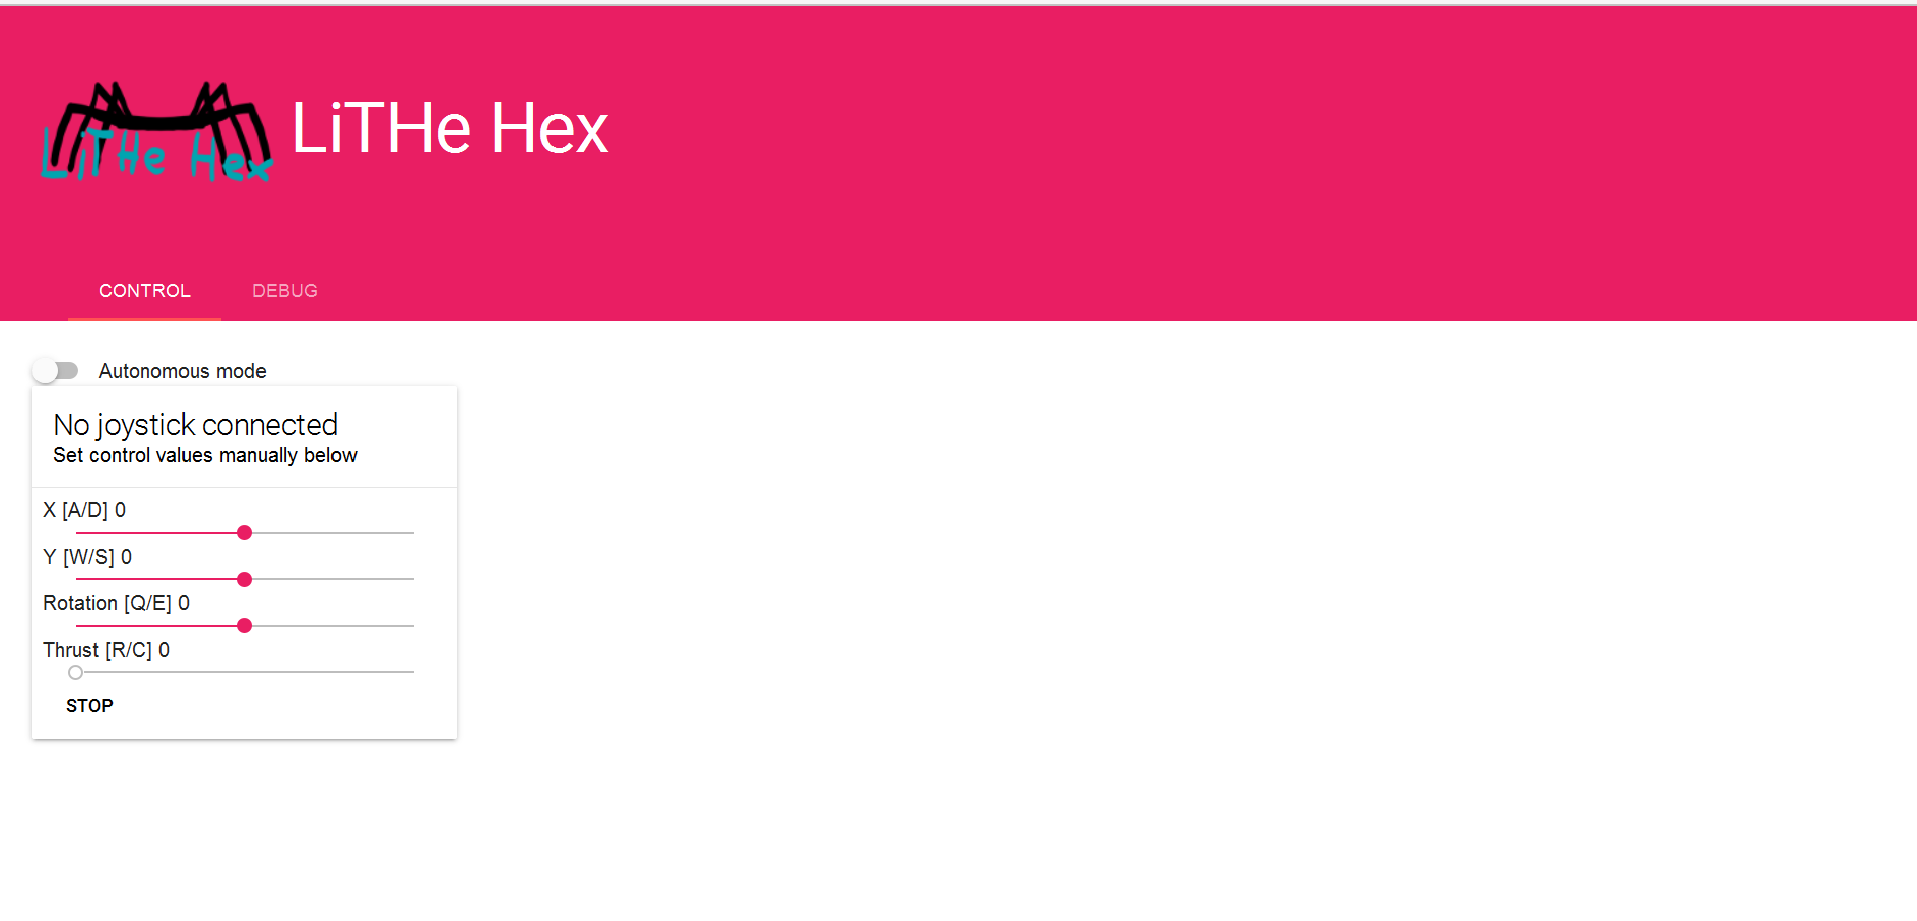
\includegraphics[width=0.5\linewidth]{images/gui-front.png}
		\caption{Det grafiska gränssnittet för control\label{fig:gui-front}}
	\end{figure}
	
	\label{gui:debug}
	\subsection{Debug}
	När man öppnat debug så finns det nio stycken olika grafer som visar olika sensordata för roboten vid det här tillfället. Graferna uppdateras tio gånger i sekunden för de nya värden som kommer in. Se figur \ref{fig:gui-debug} för hur debug sidan ser ut.
	
	\begin{figure}[h]
		\centering
		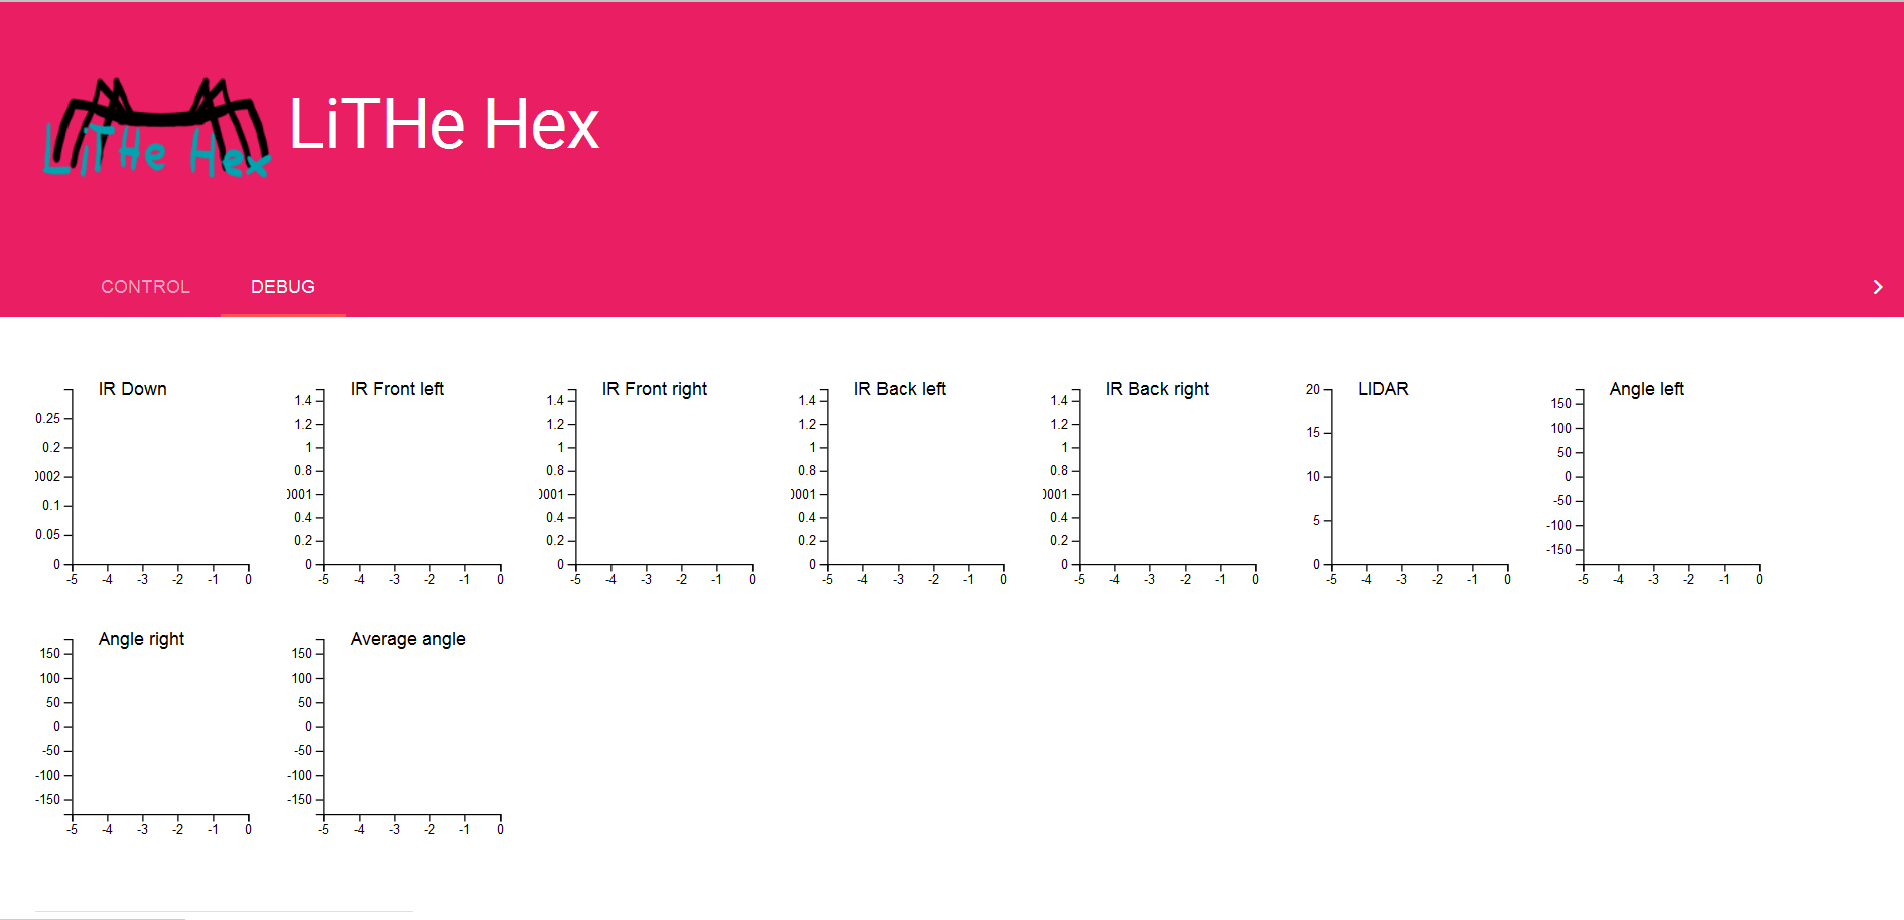
\includegraphics[width=0.5\linewidth]{images/gui-debug.png}
		\caption{Det grafiska gränssnittet för control\label{fig:gui-debug}}
	\end{figure}
	
	% TODO: Ta med om man behöver uppdatera t.ex. phoenix eller liknande?

\end{document}
